\section{$H_{\infty}$ control}
In this section we show how to design a $H_{\infty}$ controller for this system. The augmented plant consists in three shaping functions which are in charge of designing the desired closed loop sensitivities.\\

\begin{figure}[H]
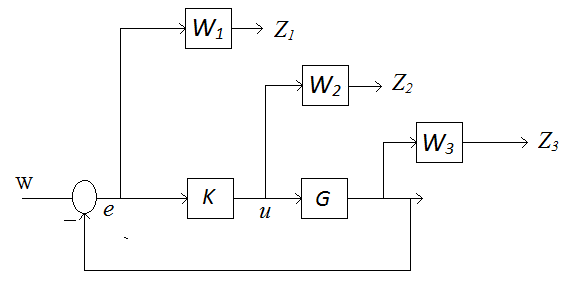
\includegraphics[width=0.5\textwidth]{img/hinf_scheme.png}
\caption{Augmented plant.}
\end{figure}

Each function has three degrees of freedom: low frequency gain, cross-over frequency and high frequency gain. The most important one is the cross-over frequency which defines the closed loop bandwidth of the system; in our case, we are aiming at a response time of about one second which corresponds to a cross-over frequency of 1 Hz ($\omega=2\pi$). The gains are tuned so to obtained the desired low and high frequency disturbance rejection, but they are not very critical for this application. The crucial function in our application is the sensitivity wrt the control input because our actuator constrains us to work in the range $\pm 5V$; hence, we need to give more weight to penalize the control effort and obtain a feasible action; this last process is performed by an iteration process of trial&error: given a shape, we test the correspondant controller on simulink and check how the control input behaves; if the input saturate then we need to weight more the effort.\\

\begin{figure}[H]
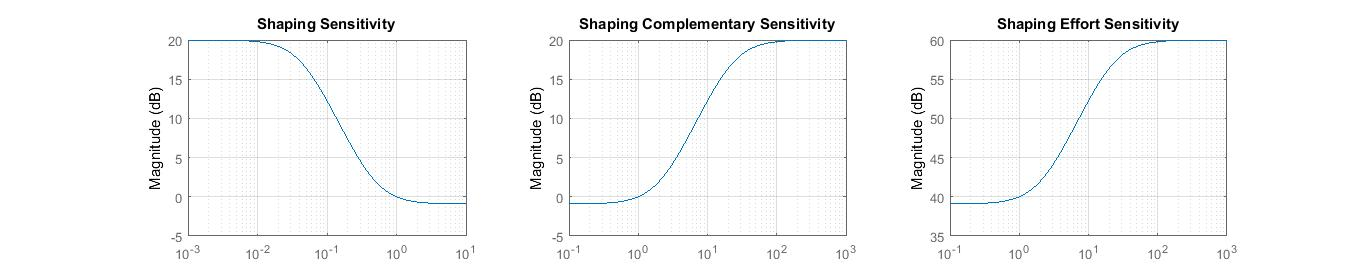
\includegraphics[width=0.5\textwidth]{img/hinf_shapes.jpg}
\caption{Shaping functions.}
\end{figure}

The controller output of the $H_{\infty}$ design has as many poles as the augmented plant; in our case, the plant has 3 poles (two from the cart and one from the motor) and so the shaping functions (one pole each), thus the final controller is a 6th order transfer function. Since we previously saw that the loopshaping technique achieves good performances with a 3rd order, it is interesting to investigate the option of reducing the complexity of the controller. With this aim, we compute the singular values of the Hankel matrix in order to see how much information is contained by every degree. It turns out that only the first order of complexity brings enough information and can approximate the controller in the bandwidth of interest. In practice, approximating to the third order is a robust solution which will not perturb for sure the theoretical results.

\begin{figure}[H]

\begin{subfigure}{0.49\textwidth}
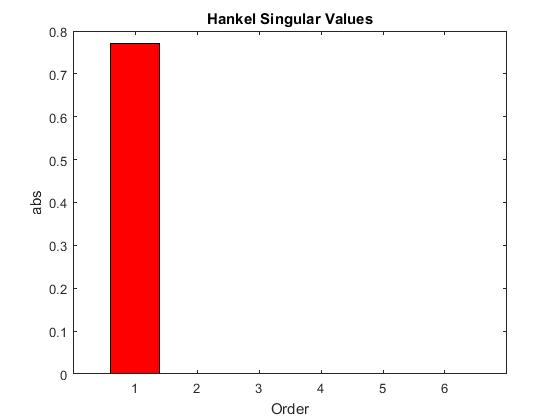
\includegraphics[width=\textwidth]{img/hinf_hankel.jpg}
\caption{Singular values of the Hankel matrix.}
\end{subfigure}

\begin{subfigure}{0.49\textwidth}
\includegraphics[width=\textwidth]{img/hinf_reduce.jpg}
\caption{Approximation with only the first order.}
\end{subfigure}

\end{figure}

%Confronto con loopshaping.

Test.
